\section{Experiments}
\label{sec:experiments}


\begin{table*}[t]
\label{table-main-comparison}
	\begin{center}
\vspace{-0.30cm}
		\caption{Quantitative comparison with SOTA methods on VBench, temporal consistency, camera accuracy, and view synchronization.}
\vspace{-0.30cm}
		\label{tab_merged_eval}
		\setlength\tabcolsep{3.2pt} % Keep small for fitting
 	\centering
 	\resizebox{\textwidth}{!}{ % Use \textwidth to fit the wide table
		\begin{tabular}{lcccccc|c|cc|ccc}
			\toprule
			\multirow{2}{*}{Method}
            & \multicolumn{6}{c|}{VBench Quality}
            & \multicolumn{1}{c|}{Temporal Consistency}
            & \multicolumn{2}{c|}{Camera Accuracy}
            & \multicolumn{3}{c}{View Synchronization} \\
     	\cmidrule(lr){2-7}
     	\cmidrule(lr){8-8}
     	\cmidrule(lr){9-10}
     	\cmidrule(lr){11-13}
            & \makecell[c]{Aesthetic $\uparrow$} & \makecell[c]{Imaging $\uparrow$} & \makecell[c]{Flickering $\uparrow$} & \makecell[c]{Smoothness $\uparrow$} & \makecell[c]{Subject $\uparrow$} & \makecell[c]{Background $\uparrow$}
			& CLIP-F $\uparrow$
			& RotErr $\downarrow$
			& TransErr $\downarrow$
			& Mat. Pix $\uparrow$
			& FVD-V $\downarrow$
			& CLIP-V $\uparrow$ \\
		\midrule

	\trajectorycrafter{} (49 frames) & 52.69 & \textbf{59.67} & 96.97 & 99.03 & 93.78 & 95.13 & 98.80 &  \textbf{2.26} & 3.03 & 1851.80 & 582.56 & 92.40 \\
	\textbf{Ours} (49 frames) & \textbf{52.72} & 57.81 & \textbf{97.43} & \textbf{99.24} & \textbf{95.09} & \textbf{95.62} & \textbf{99.01} & 2.61 & \textbf{2.73} & \textbf{2737.65} & \textbf{488.22} & \textbf{94.96} \\
    \midrule
    \midrule
	\recammaster{} & 48.71 & 52.61 & \textbf{97.57} & \textbf{99.26} & 88.57 & 90.65 & 98.49 & 11.29 & 19.59 & 1314.00 & 732.52 & 88.91 \\
	\exfd{} & 49.72 & 55.76 & 97.46 & 99.08 & 91.51 & 94.78 & 98.94 & 3.94 & \textbf{4.21} & 2188.98 & 685.63 & 89.77 \\
	% \textbf{Ours} & 53.05 & 58.39 & 97.42 & 99.20 & 93.43 & 95.11 & 99.04 & 3.27 & 4.92 & 2636.07 & 595.39 & 92.94 \\
    % \midrule
    % \textbf{Ours w/o Source Video} & \textbf{53.97} & \textbf{58.92} & 97.13 & 98.99 & 93.12 & 95.03 & 98.95 & 4.82 & 11.65 & 226.01 & 662.09 & 89.97 \\
    \textbf{Ours} & \textbf{52.85} & \textbf{58.64} & 97.37 & 99.21 & \textbf{93.43} & \textbf{95.24} & \textbf{99.03} & \textbf{2.76} & 4.23 & \textbf{2720.83} & \textbf{586.24} & \textbf{93.16} \\
\bottomrule
		\end{tabular}
 	}
	\end{center}

    \vspace{-0.15in}
\end{table*}


\begin{figure*}
    \centering
    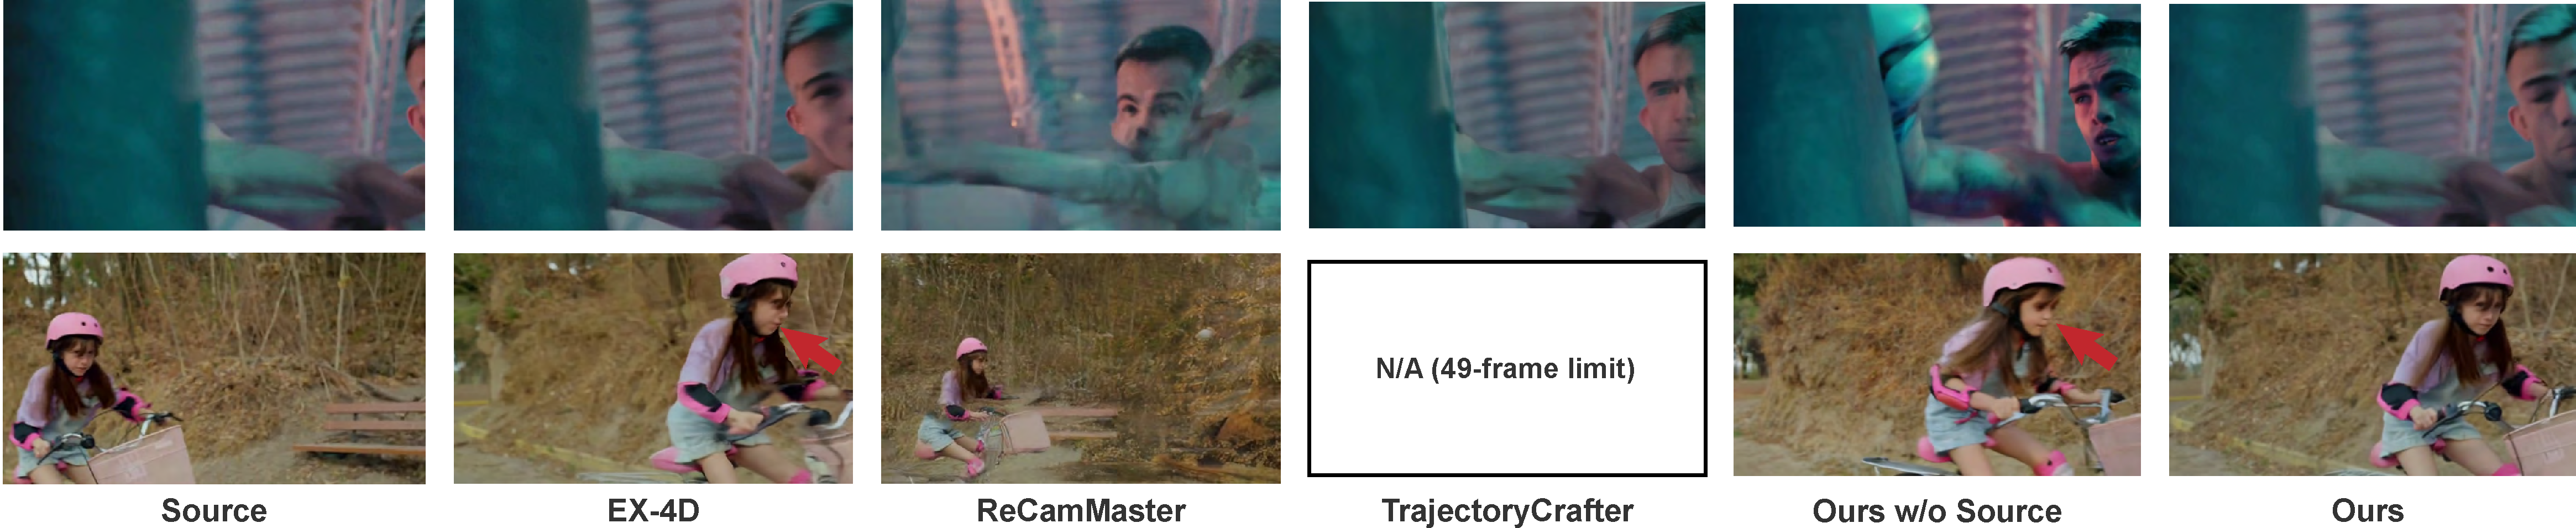
\includegraphics[width=\linewidth]{figures/comp.pdf}
    \vspace{-0.2in}
    \caption{We compare against other state-of-the-art approaches on the test set~\cite{lin2024open}. Existing approaches struggle to handle complex camera motions (e.g., shaky camera in the first example) and intricate details such as facial features in the second example (see supp. video).
    }
    \label{fig:comparisons}
    \vspace{-0.15in}
\end{figure*}


\subsection{Evaluation Setup} % Renamed for broader scope as it will include metrics, baselines etc.
\label{sec:eval_setup}

\textbf{Dataset.}
For evaluation, we constructed a representative set of 100 five-second videos from the publicly available Opensora-mixkit dataset~\cite{lin2024open}, each at 16 fps and 480p resolution. This evaluation set was systematically sampled to ensure a balanced representation of semantic concept coverage, camera motion diversity, and a mix of occluded and dis-occluded regions. More details are provided in the Supplementary Material.

\noindent\textbf{Metrics.} 
We evaluate performance across three dimensions. \textit{Camera accuracy} is measured via Rotational (RotErr) and Translational Error (TransErr) from extracted poses~\cite{camera_traj_he2024cameractrl, huang2025vipe}. \textit{View synchronization} is quantified using GIM average matching pixels (Mat. Pix.)~\cite{shen2024gim}, Fréchet Video Distance against the source video (FVD-V)~\cite{eval_unterthiner2019fvd}, and source-target frame similarity (CLIP-V). Finally, \textit{overall video quality} and temporal consistency are assessed using the VBench suite~\cite{eval_huang2024vbench} and adjacent-frame similarity (CLIP-F). More details in the Supplementary Material.

% For a comprehensive evaluation of our video reshooting model, we assess performance across three critical dimensions: \textit{camera accuracy}, \textit{view synchronization}, and \textit{overall video quality}. Camera accuracy is quantified using Rotational Error (RotErr) and Translational Error (TransErr) derived from extracted camera poses~\cite{camera_traj_he2024cameractrl, huang2025vipe}. For view synchronization, we use the image matching method GIM \cite{shen2024gim} to calculate the average number of matching pixels (Mat. Pix.) with confidence greater than a 0.5 threshold. Furthermore, we calculate the FVD-V score, which measures the Fréchet Video Distance \cite{eval_unterthiner2019fvd} between the original source videos and their corresponding generated outputs. We also present the CLIP-V score, defined as the average CLIP similarity between source and target frames at the same timestamp. Overall video quality is evaluated using the VBench benchmark's suite of perceptual metrics~\cite{eval_huang2024vbench}. To measure temporal consistency, we compute CLIP-F, the average CLIP similarity of adjacent frames in the generated videos.

% In our ablation studies, applying augmentations to the anchor video improves robustness against test-time anchor artifacts. We evaluate the coherence between the generated and source videos as the primary metric for this setting. Furthermore, we benchmark our models against state-of-the-art approaches, including \textbf{Recammaster} ~\cite{bai2025recammaster}, \textbf{TrajectoryCrafter}\cite{yu2025trajectorycrafter}, and \textbf{Ex4D} \cite{ex4d}, using \textbf{VBench} to compare overall video generation performance.


% \begin{table}[t]
% \begin{center}
%      \vspace{-0.30cm}
%      \caption{Comparison of ablation on our training strategies on temporal consistency, camera accuracy, and view synchronization.}
%      \vspace{-0.30cm}
%      \label{tab_quality_eval}
%      \setlength\tabcolsep{3.2pt}
%      \centering
%      \resizebox{0.8\linewidth}{!}{
%      \begin{tabular}{lc|cc|ccc}
%      \toprule
%      \multirow{2}{*}{Method}
%  & \multicolumn{1}{c|}{Temporal Consistency}
%  & \multicolumn{2}{c|}{Camera Accuracy}
%  & \multicolumn{3}{c}{View Synchronization} \\
%  \cmidrule(lr){2-2}
%  \cmidrule(lr){3-4}
%  \cmidrule(lr){5-7}
%  & CLIP-F $\uparrow$
%  & RotErr $\downarrow$
%  & TransErr $\downarrow$
%  & Mat. Pix $\uparrow$
%  & FVD-V $\downarrow$
%  & CLIP-V $\uparrow$ \\
%  \midrule

%  Baseline (w/ self-attn)
%  & 99.04 & 3.27 & 4.92 & 2636.07 & 595.39 & 92.94 \\
%  \midrule
%  \quad - Reference video
%  & 98.95 & 4.82 & 11.65 & 226.02 & 662.09 & 89.97 \\
%  \midrule

%  \quad + Random Color Background Anchor Videos
%  & 99.03 & 2.92 & 4.30 & 2610.26 & 593.77 & 92.78 \\

% \quad + Fluorescent Background Anchor Videos
%  & 99.02 & 3.16 & 4.78 & 2627.12 & 571.06 & 92.68 \\
%  \midrule

%  \quad + Gaussian Noise injected on Latent
%  & 98.99 & 2.81 & 5.05 & 2586.63 & 605.93 & 91.70 \\
 
%  \quad + 3D Noise injected to Anchor Video
%  & 99.02 & \textbf{2.49} & 4.95 & 2624.24 & 598.67 & 92.88 \\
%  \midrule

% \quad + Auxiliary loss
%         & 99.02 & 2.76 & 4.98 & 2627.68 & \textbf{562.94} & 92.93 \\

% \quad + LoRA
%         & \textbf{99.05} & 2.85 & \textbf{4.17} & 2615.47 & 578.91 & \textbf{92.98} \\

% \quad + Random Query
%         & 99.03 & 3.36 & 4.52 & 2618.16 & 571.74 & 92.83 \\

%  \midrule
%  \textbf{Ours} & 99.03 & 2.76 & 4.23 & \textbf{2720.83} & 586.24 & 93.16 \\
%  \bottomrule
%  \end{tabular}
%  }
% \end{center}

%     \vspace{-0.25in}
% \end{table}



\subsubsection{Baseline Methods}
\label{sec:baselines}

We compare our approach against recent state-of-the-art video reshooting methods. We evaluate against \recammaster{}~\cite{bai2025recammaster}, which is conditioned on a source video and a target camera trajectory. We also compare against \exfd{}~\cite{ex4d}, an approach that solely relies on anchor videos, and \trajectorycrafter{}~\cite{yu2025trajectorycrafter}, which is conditioned on both anchor videos and a source video. For a fair comparison with \trajectorycrafter{}, which natively generates 49-frame videos, all metrics are computed on the first 49 frames of both their outputs and our corresponding generations.

\subsection{Comparisons with State-of-the-Art Methods}
\label{sec:comparisons}

Our approach consistently outperforms existing state-of-the-art methods in dynamic video reshooting. Quantitatively, as detailed in Table~\ref{tab_merged_eval}, our model demonstrates leading performance across most metrics. We achieve superior overall video quality, temporal consistency, and view synchronization while maintaining highly competitive camera accuracy and robust geometric fidelity against all baselines.

Qualitatively, Figure~\ref{fig:comparisons} illustrates two dynamic scenes from the test set to compare our output against existing baselines. The output quality of \recammaster{} is notably poor, which is partially due to the publicly released checkpoint being a limited 1.3B parameter model. For anchor-only methods like \exfd{}, the lack of direct source video conditioning causes the warping artifacts present in the anchor video to carry over directly into the generated output. Similarly, \trajectorycrafter{} struggles to maintain high visual fidelity due to limitations within its underlying training setup. To further validate the necessity of our architecture, we visualize our model trained without source video conditioning (`Ours w/o Source'). Much like \exfd{}, omitting the source video prevents the model from capturing and preserving the intricate details of the original footage.

Consequently, existing methods struggle with complex camera motions (e.g., shaky footage) and fine facial details. In contrast, our full method leverages implicit 4D routing to handle these challenges, producing high-fidelity outputs that preserve the original content. More comparisons on challenging trajectories are in the Supplementary Material.






\begin{figure}[ht]
    \centering
    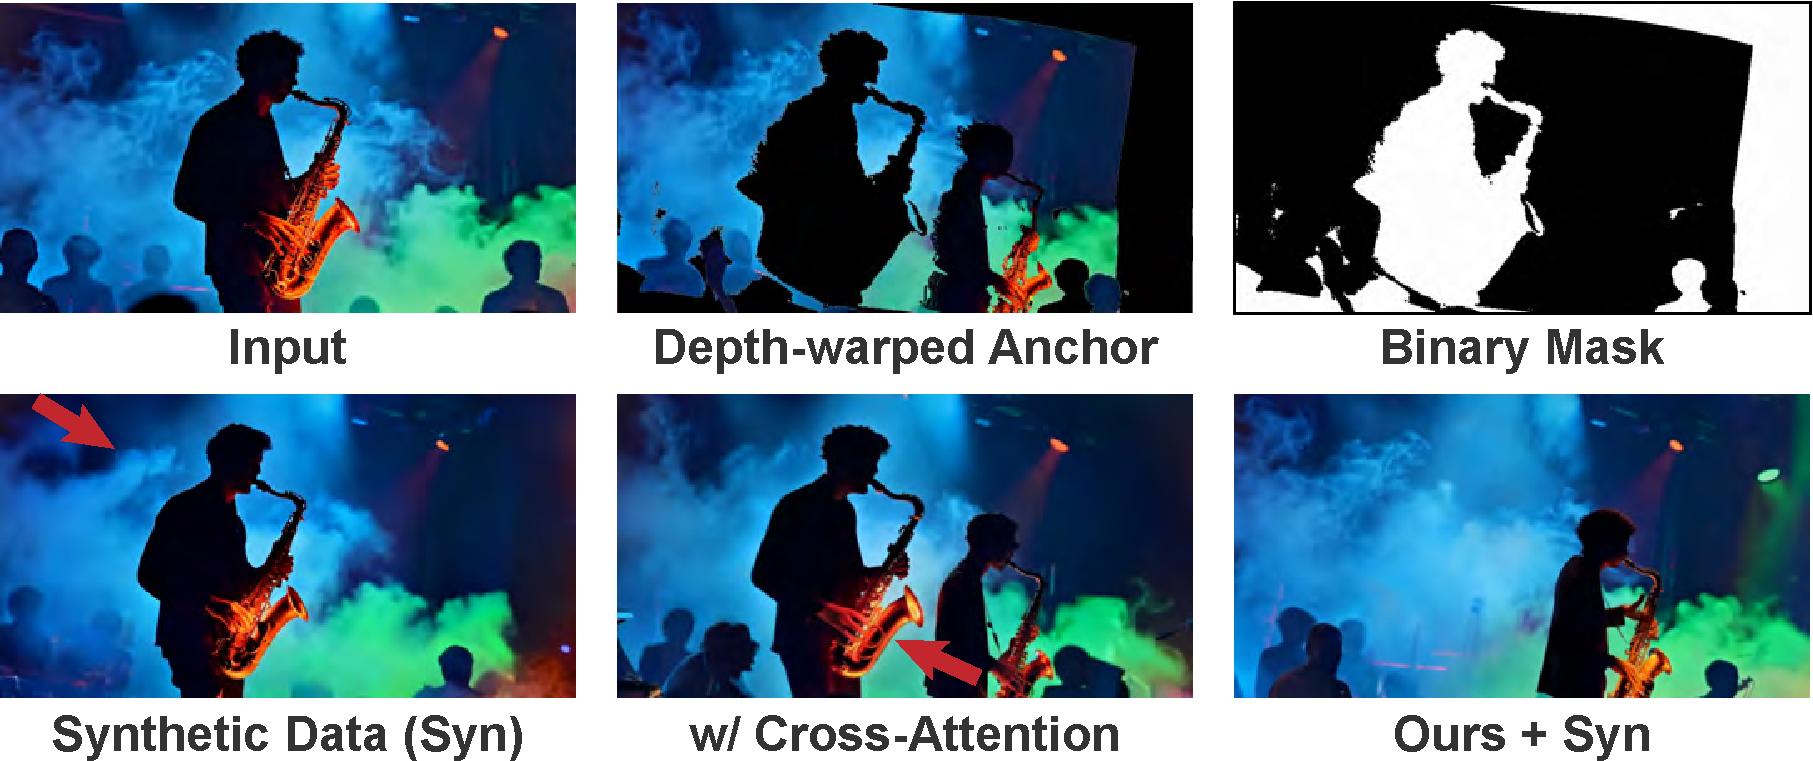
\includegraphics[width=\linewidth]{figures/ablation_comp.pdf}
    \vspace{-0.15in}
    \caption{We evaluate critical architectural and data components on a complex scene featuring moving smoke and colored lighting. The \textit{Synthetic Data Only} model fails to capture the intricate dynamics of the smoke. The \textit{Cross-Attention} model fails to preserve fine source details, such as the texture of the saxophone. Both baselines struggle to accurately align with the anchor condition, resulting in structural hallucinations. In contrast, our model faithfully tracks the anchor while preserving high-fidelity textures and complex scene dynamics.}
    \label{fig:ablation_comp}
    % \vspace{-0.15in}
\end{figure}
\begin{table}[ht]
\begin{center}
     \vspace{-0.10cm}
     \caption{Quantitative ablation of our training strategies, evaluating camera accuracy and view synchronization.}
     \vspace{-0.20cm}
     \label{tab_quality_eval}
     \setlength\tabcolsep{3.2pt}
     \centering
     \resizebox{\linewidth}{!}{
     \begin{tabular}{l|cc|ccc}
     \toprule
     \multirow{2}{*}{Method}
 & \multicolumn{2}{c|}{Camera Accuracy}
 & \multicolumn{3}{c}{View Synchronization} \\
 \cmidrule(lr){2-3}
 \cmidrule(lr){4-6}
 & RotErr $\downarrow$
 & TransErr $\downarrow$
 & Mat. Pix $\uparrow$
 & FVD-V $\downarrow$
 & CLIP-V $\uparrow$ \\
 \midrule

 Baseline (w/ self-attn)
 & 3.27 & 4.92 & 2636 & 595.39 & 92.94 \\
 \midrule
 \quad - Source Video
 & 4.82 & 11.65 & 226 & 662.09 & 89.97 \\
 \midrule

 \quad + Gaussian Noise in Latent
 & 2.81 & 5.05 & 2586 & 605.93 & 91.70 \\
 
 \quad + 3D Noise in Anchor
 & 2.49 & 4.95 & 2624 & 598.67 & 92.88 \\
 \midrule

\quad w/ cross-attn
        & 3.53 & 4.31 & 1766 & 626.37 & 91.64 \\
        
\quad + Auxiliary Loss
        & 2.76 & 4.98 & 2627 & 562.94 & 92.93 \\

\quad + LoRA
        & 2.85 & 4.17 & 2615 & 578.91 & 92.98 \\

\quad + Random Query
        & 3.36 & 4.52 & 2618 & 571.74 & 92.83 \\
        
\quad + Fluorescent Background Anchor
 & 3.16 & 4.78 & 2627 & 571.06 & 92.68 \\

 \midrule
 w/ Synthetic Data (Syn) & 3.70 & 5.04 & 1746 & 608.03 & 91.86 \\
 w/ Monocular Videos (\textbf{Ours}) & 2.76 & 4.23 & 2720 & 586.24 & 93.16 \\
 \textbf{Ours + Syn} & 3.36 & 3.66 & 2577 & 587.91 & 92.64 \\
 \bottomrule
 \end{tabular}
 }
\end{center}
    \vspace{-0.25in}
\end{table}


\subsection{Ablations}
\label{sec:ablations}

We conduct targeted ablation studies to quantify the impact of our core architectural choices and training data strategies against a defined baseline. Our baseline configuration uses a black background for the anchor video, processes the source video via token concatenation through the self-attention layers, and is trained exclusively on monocular videos without any additional augmentations. Detailed quantitative results are presented in Table~\ref{tab_quality_eval}, alongside some qualitative comparisons in Figure~\ref{fig:ablation_comp}.

\noindent\textbf{Hybrid Dataset.} We validate our data strategy by evaluating models trained exclusively on synthetic data (`w/ Synthetic Data (Syn)'), purely on monocular videos (`Ours'), and our 15\% mixture (`Ours + Syn'). While the synthetic-only model achieves reasonable camera alignment, it severely degrades texture fidelity. Qualitatively (Figure~\ref{fig:ablation_comp}), the synthetic-only baseline fails to capture complex real-world dynamics, such as smoke moving under colored lighting, and struggles with anchor alignment in complex scenes, leading to structural hallucinations. In contrast, our full hybrid approach (`Ours + Syn') seamlessly preserves these intricate dynamics, confirming that grounding the model in real-world triplets is essential for physical realism. Furthermore, as demonstrated in Figure~\ref{fig:hybrid_ablation}, while the purely monocular model (`Ours') excels under moderate motion, incorporating the synthetic mixture (`Ours + Syn') is critical for enabling robust geometric control during extreme, out-of-distribution camera trajectories.

\noindent\textbf{Conditioning Architecture.} We evaluate the integration of the source video condition by comparing our token concatenation strategy against a dedicated cross-attention mechanism (`w/ cross-attn'). Cross-attention performs significantly worse across all quantitative metrics. Visually (Figure~\ref{fig:ablation_comp}), this variant fails to reliably pass fine details from the source video to the generated output, completely losing the correct texture on the saxophone. It also exhibits poor anchor alignment. In contrast, our token concatenation approach natively leverages the pre-trained self-attention layers, yielding vastly superior view synchronization and structural accuracy.

\noindent\textbf{Technical Augmentations.} Beyond core architecture, we validate our technical augmentations in Table~\ref{tab_quality_eval}. Key findings confirm the critical roles of our fluorescent anchor background, 3D-aware noise injection for strict geometric guidance without texture copying, the auxiliary source token reconstruction loss for content fidelity, LoRA fine-tuning for generalization, and random anchor reference frame warping for robustness.
